\documentclass{standalone}

% graphics
\usepackage[usenames,dvipsnames]{xcolor}
\usepackage{tikz}
\usepackage{pgfplots}
\usepackage{siunitx}
\usepgfplotslibrary{colorbrewer}

\begin{document}

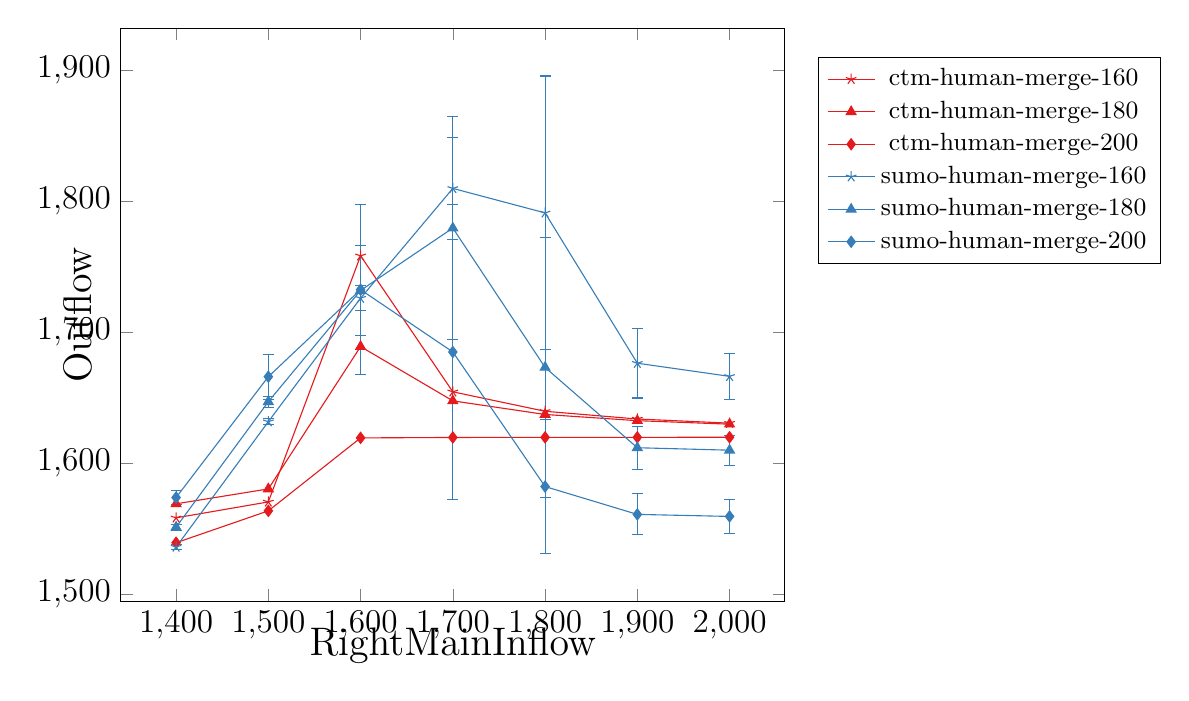
\begin{tikzpicture}[scale=1]
  \pgfplotsset{
      scale only axis,
      every x tick label/.append style={font=\large},
      every y tick label/.append style={font=\large},
	legend style={at={(1.05,0.95)},anchor=north west}
  }

\pgfplotsset{cycle list/Set1-6}

\pgfplotscreateplotcyclelist{mycolorlist}{%
	 index of colormap=0 of Set1-6,  every mark/.append style={fill=Set1-B}, mark=star, error bars/.cd, y dir=both, y explicit\\
	 index of colormap=0 of Set1-6, densely dashed every mark/.append style={fill=Set1-B}, mark=triangle*, error bars/.cd, y dir=both, y explicit\\
	 index of colormap=0 of Set1-6, dashed every mark/.append style={fill=Set1-B}, mark=diamond*, error bars/.cd, y dir=both, y explicit\\
	 index of colormap=1 of Set1-6,  every mark/.append style={fill=Set1-B}, mark=star, error bars/.cd, y dir=both, y explicit\\
	 index of colormap=1 of Set1-6, densely dashed every mark/.append style={fill=Set1-B}, mark=triangle*, error bars/.cd, y dir=both, y explicit\\
	 index of colormap=1 of Set1-6, dashed every mark/.append style={fill=Set1-B}, mark=diamond*, error bars/.cd, y dir=both, y explicit\\
}
\begin{axis}[
    legend style={font=\small},
	ylabel={\Large Outflow},
	x label style={at={(axis description cs:0.5,-0.03)},anchor=north},
	y label style={at={(axis description cs:-0.030,0.5)}, anchor=south},
	%xticklabel style = {font=\small,xshift=0.5ex},
	xlabel={\Large RightMainInflow},
	%legend columns=15,
	legend columns=1,
	%transpose legend,
	/tikz/column /.style={
                column sep=5pt,
            },
	cycle list name=mycolorlist
]
%end of axis
\addplot table [x=a, y=b] {
a	 b	 c
1400 1558.4399999999807 
1500 1570.5758878098532
1600 1758.24
1700 1654.5315569525305
1800 1639.699555047557
1900 1633.8077752853937
2000 1630.6352486042115
};
\label{ctm-human-merge-160}


\addplot table [x=a, y=b] {
a	 b	 c
1400 1569.1377955567793
1500 1580.4861450169294 
1600 1689.0349310665047
1700 1647.6511601325865
1800 1637.2660868322826
1900 1632.5361735290298
2000 1629.8627368936695
};
\label{ctm-human-merge-180}

\addplot table [x=a, y=b] {
a	 b	 c
1400 1539.4513763215234 
1500 1563.7588553640305
1600 1619.3999428517002
1700 1619.7299678533159
1800 1619.8056896113792
1900 1619.8349783900273
2000 1619.8799839978665
};
\label{ctm-human-merge-200}

\addplot table [x=a, y=b, y error=c] {
a	 b	 c
1400 1536.19 1.77 
1500 1631.77 2.21  
1600 1725.95 9.42
1700 1809.65 39.00 
1800 1790.96 104.43 
1900 1676.34 26.52 
2000 1666.33 17.66   
};
\label{sumo-human-merge-160}

\addplot table [x=a, y=b, y error=c] {
a	 b	 c
1400 1551.28 2.28
1500 1647.00 4.21 
1600 1731.85 34.59   
1700 1779.41 85.19 
1800 1673.14 99.30 
1900 1611.90 16.39 
2000 1610.03 11.35   
};
\label{sumo-human-merge-180}

\addplot table [x=a, y=b, y error=c] {
a	 b	 c
1400 1573.92 5.36  
1500 1666.08 17.25    
1600 1732.43 64.95  
1700 1684.91 112.53  
1800 1582.31 50.93
1900 1561.07 15.63  
2000 1559.52 12.70
};
\label{sumo-human-merge-200}


\addlegendimage{/pgfplots/refstyle=ctm-human-merge-160}
\addlegendentry{ctm-human-merge-160}

\addlegendimage{/pgfplots/refstyle=ctm-human-merge-180}
\addlegendentry{ctm-human-merge-180}

\addlegendimage{/pgfplots/refstyle=ctm-human-merge-200}
\addlegendentry{ctm-human-merge-200}

\addlegendimage{/pgfplots/refstyle=sumo-human-merge-160}
\addlegendentry{sumo-human-merge-160}

\addlegendimage{/pgfplots/refstyle=sumo-human-merge-180}
\addlegendentry{sumo-human-merge-180}

\addlegendimage{/pgfplots/refstyle=sumo-human-merge-200}
\addlegendentry{sumo-human-merge-200}


\end{axis}
\end{tikzpicture}
\end{document}
